\chapter{Resultados} \label{sec:results}

Após a execução de grande número de episódios para treinamento dos modelos
propostos foram separados em planilhas as quantidades de gols resultantes para
cada bloco de 3000 ciclos para cada um. Em cima desse registro foi feita uma
média geral, uma média dos primeiros 100 registros e uma média de apenas os
últimos 100 registros, levando em conta que se
espera que tenha havido uma melhora na defesa de cada um.

Na Tabela \ref{tab:results} estão listados os modelos e as médias calculadas e
por fim o valor para comparação do time original. Uma comparação visual é
ilustrada pela Figura \ref{img:averages}.

\begin{table}[hbt]
    \centering
    \begin{tabular}{c|c|c|c}
        Modelo & Média Geral & Média dos primeiros 100 blocos & Média dos últimos 100 blocos \\ \hline
        Modelo \ref{model:old} & 44,08 & 44,09 & 44,11  \\
        Modelo \ref{model:2cycles} & 40,40 & 40,21 & 35,75 \\
        Modelo \ref{model:1cycle} & 39,13 & 44,1 & 37,85 \\
        Modelo \ref{model:simple} & 44,68 & 44,4 & 44,78 \\ \hline
        Original &  26,45\\
    \end{tabular}
    \caption{\textit{Resultados}}
    \label{tab:results}
\end{table}

\imagem{.4}{averages}{Médias finais em comparação ao original}{O Autor}

A observação da Tabela \ref{tab:results} faz com que seja possível perceber que
os modelos com melhor evolução, ou alguma evolução, são os Modelos
\ref{model:2cycles} e \ref{model:1cycle}. Por conta desta observação foram
realizados um número maior de execuções nos mesmos para que fossem 
traçados gráficos (Figura \ref{img:graph}) cruzando o número de blocos executados no teste e o número de
gol sofridos no último bloco juntamente com a curva de tendência linear formada
por este cruzamento de ambos modelos para que se possa ser feito a visualização
do melhoramento dos mesmos.

\begin{figure}[!htb]
\centering
    \caption{\label{img:graph} Gráficos de Modelos \ref{model:2cycles} e \ref{model:1cycle}}
    \subcaptionbox{\label{img:2cycles} Modelo \ref{model:2cycles}}{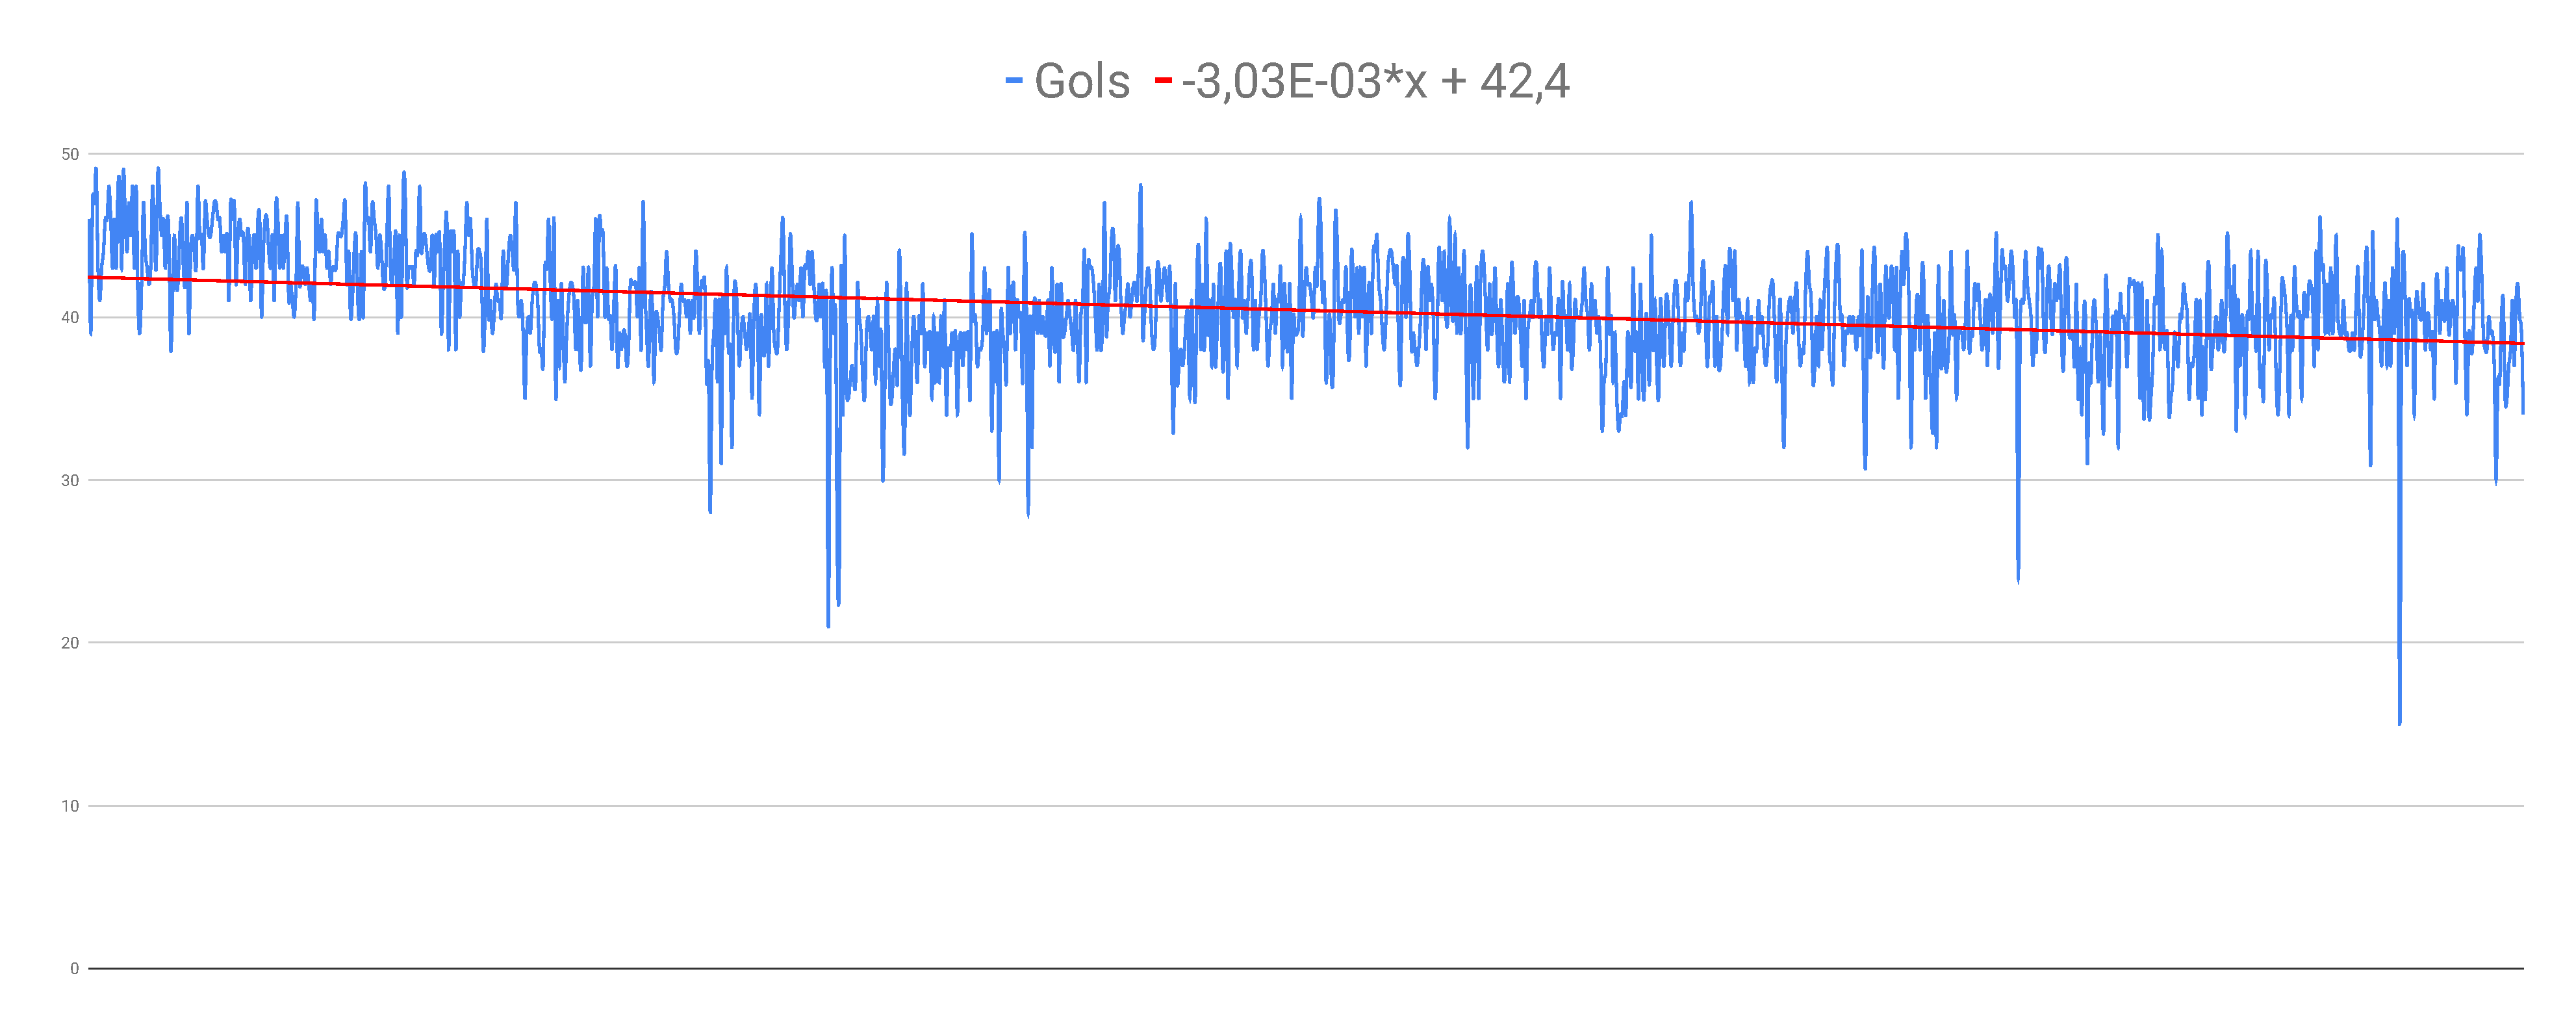
\includegraphics[scale=.235]{img/2cycles}}\qquad
    \subcaptionbox{\label{img:1cycle} Model \ref{model:1cycle}}{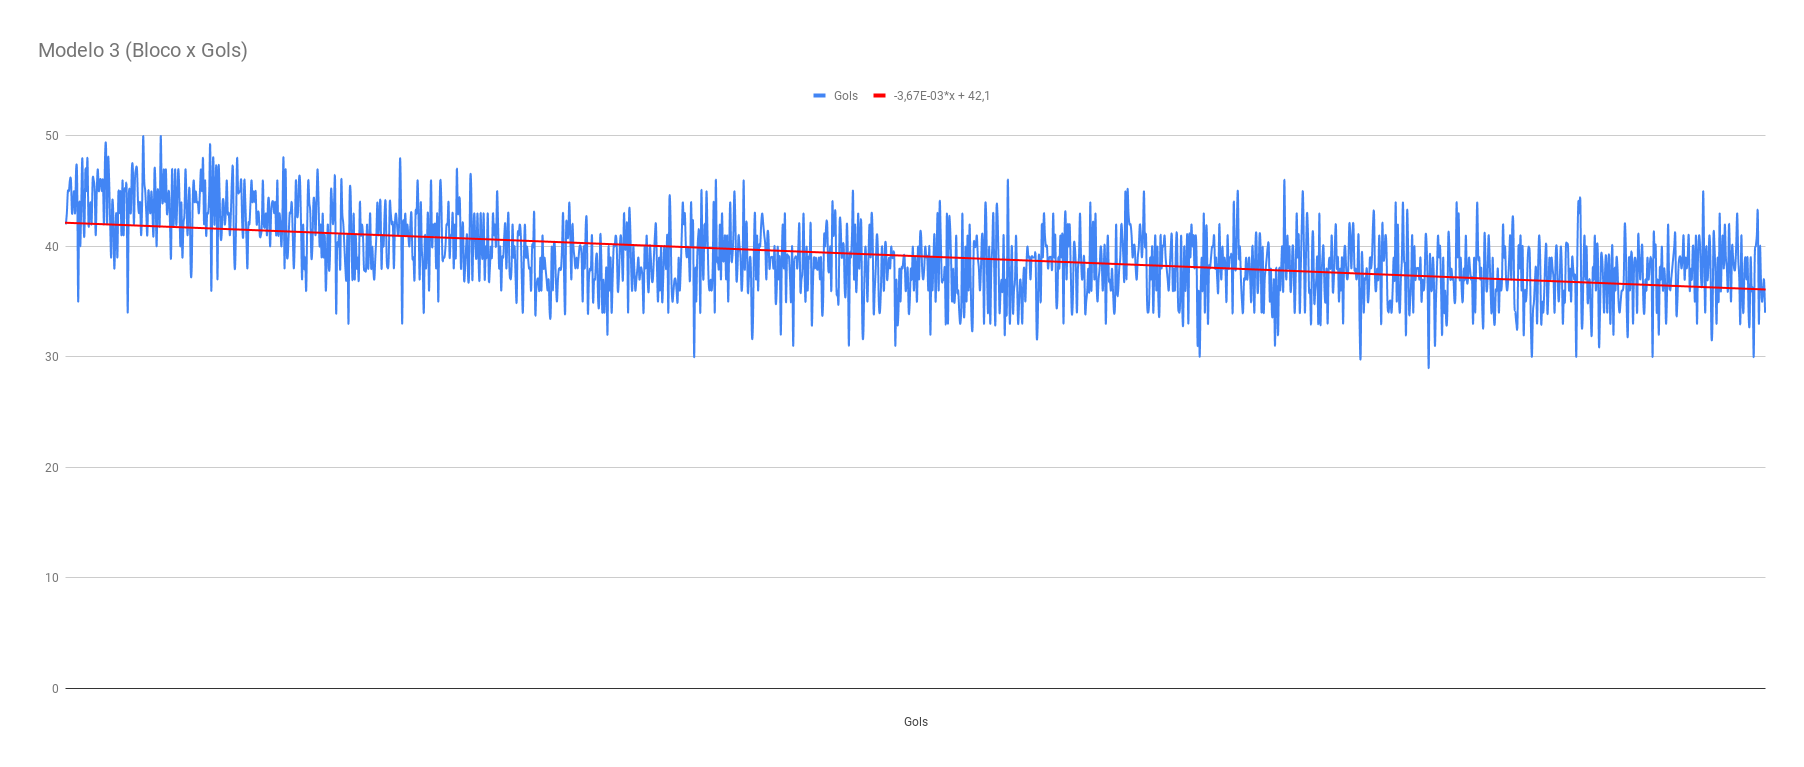
\includegraphics[scale=.25]{img/1cycle}}
    \vspace{1.5em}
    \legend{\textbf{Fonte:} O Autor}
\end{figure}

Os gráficos foram traçados com auxílio da ferramenta de planilhas Google Sheets\footnote{https://docs.google.com/spreadsheets} que
permitiu a captura da equação da curva de tendência traçada. O Modelo
\ref{model:2cycles} é representado pela equação \ref{eq:2cycles} e o Modelo
\ref{model:1cycle} é representado pela Equação \ref{eq:1cycle}, onde $G$
representa a média de gols sofridos por bloco e $b$ o número de blocos executados.

\begin{equation}
    \label{eq:2cycles}
    G=-3,03\times 10^{-3}\times b+42,4
\end{equation}

\begin{equation}
    \label{eq:1cycle}
    G=-3,67\times 10^{-3} \times b+42,1
\end{equation}